\begin{enumerate}
	\item Let $y = Av \in \im(A)$ and $x \in \ker(A^T)$. Then $$y^Tx = (Av)^Tx = v^TA^Tx = v^T(A^Tx)= 0.$$ 
Apply this to $C = A^T$ to show the other results.
\item  		Let us consider
$$A = \begin{pmatrix}1&2\\3&6\end{pmatrix}	,~~~~A^\top= \begin{pmatrix}1&3\\2&6\end{pmatrix}.$$
	Then we find\\
	\begin{minipage}[t]{0.48\textwidth} \small
		\begin{align*}
		\im(A) &= \text{span} \begin{pmatrix}1\\3\end{pmatrix}\\
		\ker(A) &= \{x\in\R^2: Ax = 0\}\\
		&= \{x\in\R^2:  x_1\begin{pmatrix}1\\3\end{pmatrix} +  x_2\begin{pmatrix}2\\6\end{pmatrix} = 0\} \\
		&= \{x\in\R^2: 1x_1 + 2x_2 = 0\} \\
		&= \{x\in\R^2: x_1 = - 2x_2\} \\
		&= \text{span} \begin{pmatrix}-2\\1\end{pmatrix}
		\end{align*}
	\end{minipage}
	\begin{minipage}[t]{0.48\textwidth} \small
		\begin{align*}
		\im(A^\top) &= \text{span} \begin{pmatrix}1\\2\end{pmatrix}\\
		\ker(A^\top) &= \{x\in\R^2: Ax = 0\}\\
		&= \{x\in\R^2: 1x_1 + 3x_2 = 0\}\\
		&= \{x\in\R^2:  x_1 = - 3x_2 \}\\
		&= \text{span} \begin{pmatrix}-3\\1\end{pmatrix}
		\end{align*}
	\end{minipage}
	~\\
	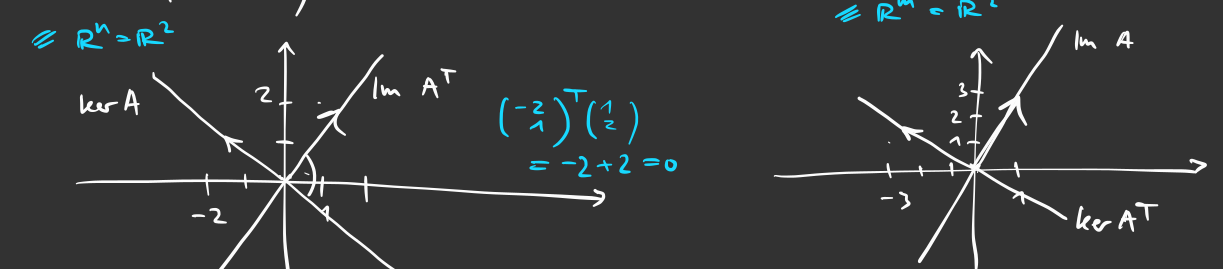
\includegraphics[width=0.9\linewidth]{ex-bigPicture-LA}
\end{enumerate}
